%
% notes.tex -- Template für standalone TIKZ Bilder
%
% (c) 2019 Prof Dr Andreas Müller, Hochschule Rapperswil
%
\documentclass[tikz]{standalone}
\usepackage{amsmath}
\usepackage{times}
\usepackage{txfonts}
\usepackage{pgfplots}
\usepackage{csvsimple}
\usetikzlibrary{arrows,intersections,math}
\begin{document}
\begin{tikzpicture}[>=latex]

\node at (1.5,{0.375*11}) {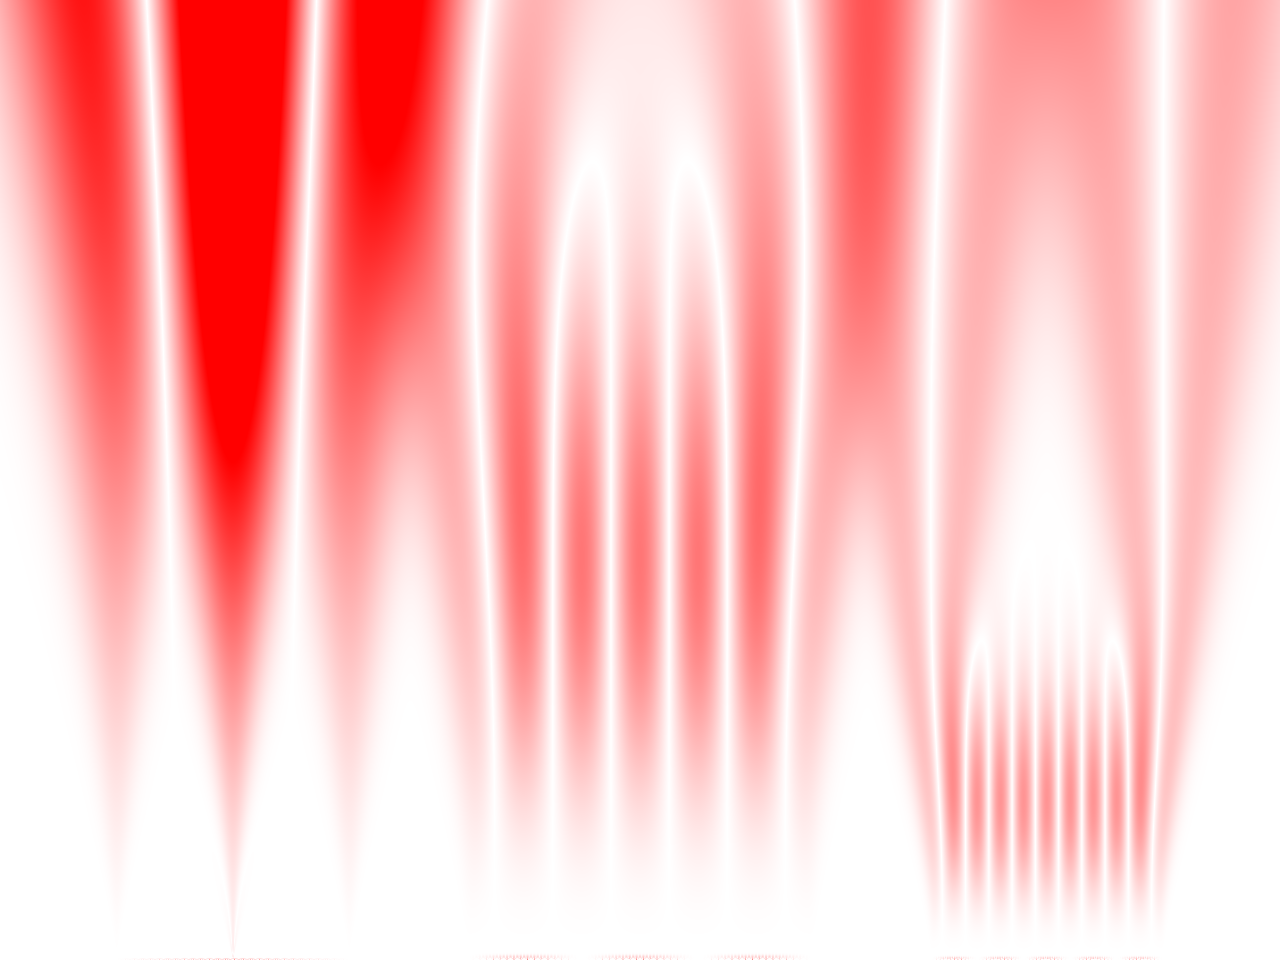
\includegraphics[width=11cm]{notes.png}};

\draw[->,line width=1pt] (-4.1,0)--(7.3,0) coordinate[label={$b$}];
\draw[->,line width=1pt] (0,-0.1)--(0,{0.75*11+0.3}) coordinate[label={right:$a$}];

\draw[line width=1pt] (-0.1,{0.3333*0.75*11})--(0.1,{0.3333*0.75*11});
\draw[line width=1pt] (-0.1,{0.6666*0.75*11})--(0.1,{0.6666*0.75*11});
\draw[line width=1pt] (-0.1,{1.0000*0.75*11})--(0.1,{1.0000*0.75*11});

\node at (-0.1,{0.3333*0.75*11}) [left] {$0.2$};
\node at (-0.1,{0.6666*0.75*11}) [left] {$0.4$};
\node at (-0.1,{1.0000*0.75*11}) [left] {$0.6$};

\foreach \x in {-4,...,7}{
	\draw[line width=1pt] ({\x},-0.1)--({\x},0.1);
}
\foreach \x in {0,...,7}{
	\node at ({\x},-0.1) [below] {$\x$};
}
\foreach \x in {-4,...,-1}{
	\node at ({\x},-0.1) [below] {$\x$};
}

\end{tikzpicture}
\end{document}

